\documentclass{article}

% if you need to pass options to natbib, use, e.g.:
% \PassOptionsToPackage{numbers, compress}{natbib}
% before loading nips_2016
%
% to avoid loading the natbib package, add option nonatbib:
% \usepackage[nonatbib]{nips_2016}

%\usepackage{nips_2016}

% to compile a camera-ready version, add the [final] option, e.g.:
\usepackage[final]{nips_2016}

\usepackage[utf8]{inputenc} % allow utf-8 input
\usepackage[T1]{fontenc}    % use 8-bit T1 fonts
\usepackage{hyperref}       % hyperlinks
\usepackage{url}            % simple URL typesetting
\usepackage{booktabs}       % professional-quality tables
\usepackage{amsfonts}       % blackboard math symbols
\usepackage{amsmath}
\usepackage{nicefrac}       % compact symbols for 1/2, etc.
\usepackage{microtype}      % microtypography
\usepackage{t1enc}
\usepackage{graphicx}
\usepackage{float}

\graphicspath{{./figs/}}

\title{Music generation using Deep Learning}

% The \author macro works with any number of authors. There are two
% commands used to separate the names and addresses of multiple
% authors: \And and \AND.
%
% Using \And between authors leaves it to LaTeX to determine where to
% break the lines. Using \AND forces a line break at that point. So,
% if LaTeX puts 3 of 4 authors names on the first line, and the last
% on the second line, try using \AND instead of \And before the third
% author name.

\author{
	Gábor Lant \\
	Department of Telecommunications and Media Informatics\\
	Budapest University of Technology and Economics\\
	Budapest, PA 1111 \\
	\texttt{lant.gabor98@gmail.com} \\
	\And
	Dániel M. Szalai\\
	Department of Networked Systems and Services\\
	Budapest University of Technology and Economics\\
	Budapest, PA 1111\\
	\texttt{szalaimd@gmail.com}\\
	\And
	Attila Kádár\\
	Department of Measurement and Information Systems\\
	Budapest University of Technology and Economics\\
	Budapest, PA 1111\\
	\texttt{attilaka98@gmail.com}
	%% examples of more authors
	%% \And
	%% Coauthor \\
	%% Affiliation \\
	%% Address \\
	%% \texttt{email} \\
	%% \AND
	%% Coauthor \\
	%% Affiliation \\
	%% Address \\
	%% \texttt{email} \\
	%% \And
	%% Coauthor \\
	%% Affiliation \\
	%% Address \\
	%% \texttt{email} \\
	%% \And
	%% Coauthor \\
	%% Affiliation \\
	%% Address \\
	%% \texttt{email} \\
}

\begin{document}
% \nipsfinalcopy is no longer used

\maketitle



\begin{abstract}
  In this paper we try to demonstrate how we can generate music using neural networks from sound files converted to images. The goal is to compare the performance of different types of neural networks and also different types of music to image conversions and how they affect the generated output.
\end{abstract}


\section{Problem summary}
\label{sec:summary}
Our idea was to convert our music data into pictures and then use some kind of neural network to produce similar pictures. Then we would convert our generated images back to music format and rate the quality. Originally we hoped we could use different styles of music to use as an input for our model and then it would generate a similar music but in a different style, but later we found this to be much more difficult. We will discuss this later in section~\ref{}.

\section{Data acquisition, description}
\label{sec:data}
For our data-set we had two criteria in mind: we needed .midi files and we wanted to use tracks similar to each other in style. The .midi files allow us to work with large data-sets (25- 100GB as uncompressed .wav files) without actually having to store them as .wavs thus taking up only minimal storage capacity (not counting the preprocessed files). Them being similar in style is not necessary, however we thought that it would be best for our first approach to only consider tracks from the same style. Luckily we found a well-made data-set called Magenta: Maestro~\cite{maestro}, that satisfies all our needs. Maestro is a dataset composed of over 200 hours of virtuosic piano performances.

\section{Data exploration}
\label{sec:exploration}
Our data has the following main features:
\begin{itemize}
	\item Time: Absolute time, in terms of MIDI clocks, at which this event occurs. Meta-events
	for which time is not meaningful (for example, song title, copyright information, etc.)
	have an absolute time of 0.
	\item Type/Event: Name identifying the type of the record. Record types are text consisting
	of upper and lower case letters and the underscore (``\_''), contain no embedded
	spaces, and are not enclosed in quotes.
	\item Channel: The channel identifier.
	\item Note: The currently played note (integer 21-109, a piano has 88 keys)
	\item Velocity: The matching note’s volume at the moment.
\end{itemize}
Further details at midicsv’s website~\footnote{MIDICSV: Convert MIDI File to and from CSV - Fourmilab. \url{https://www.fourmilab.ch/webtools/midicsv/}}

\section{Data preprocessing}
\label{sec:prepoc}
Here we only explain the main steps and ideas of our preprocessing, because we include a well-commented source code, that produces our actual training (70\%), validation (20\%) and test (10\%) data.

\subsection{First approach - using the midi files}
	\subsubsection{Encoding}
	We used a python package called \textbf{MidiFile} to process the midi files in the following way:
	\begin{enumerate}
		\item With the constructor of \textbf{Midifile} we can read a specific .midi file and get all the MIDI event messages presented in it. 
		\item From the aquired event messages we built a pandas dataframe which made data handling easier. The structure of the dataframe can be seen on figure \ref{fig:dframe}
		
		\begin{figure}[!htb]
			\centering
			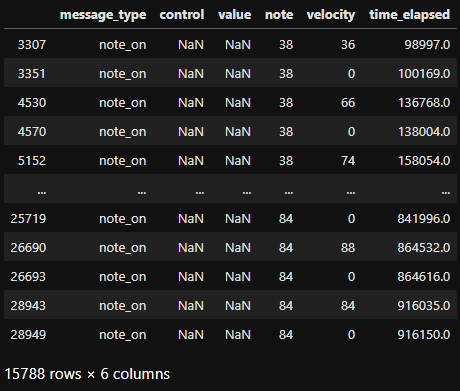
\includegraphics[width=\linewidth]{dframe.png}
			\caption{Pandas dataframe containing midi events.}
			\label{fig:dframe}
		\end{figure}
		\item The time\_elapsed column contains the same Time value as it is in the original .midi file. This column will help us to determine the starting and ending pixel of the note appearing on the generated image.
		\item We created image files, where the pitch is representsand on the y axis and the time on the x axis (we created images with size of 88x200 pixels storing approximatelly 10 seconds long pieces of music). We used three different coding methods to compare their performance: 
		\begin{itemize}
			\item In the first method we used all the 4 channels of a pixel to store different infromations about every note: its length, velocity, which instrument played that note and finally the current tempo. An example of this encoding can be seen on figure \ref{fig:encoded-1}. This encoding is very rare, since only the starting of notes are presented on these images, because the length of each note is stored in R channel. 
			\begin{figure}[!htb]
				\centering
				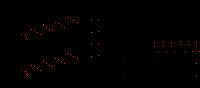
\includegraphics[width=\linewidth]{encode1.png}
				\caption{Encoding number 1.}
				\label{fig:encoded-1}
			\end{figure}
			\item The second method is very similar to the one presented above, one difference is that this encoding uses only 3 channels, because we observed that in our dataset the Tempo value is equal in every part of each song so it is not necessary to store that feature. Also in this encoding we don't store the length of notes, the value of R channel is either 125 (which means the beginning of a given note) or 255 (means that a note is sustained). So in this encoding the whole time intervall is painted where a given note is played. An example of this encoding can be seen on figure \ref{fig:encoded-2}. The index of pixels between the note shuld be painted can be determined as follows: 
				\begin{gather}
					starting\_time = tempo\times\frac{\frac{t_0}{division}}{100000} seconds \\ \nonumber
					starting\_pixel = starting\_time \times pixel\_sec \\ \nonumber
					ending\_time = tempo\times\frac{\frac{t_1}{division}}{100000} seconds \\ \nonumber
					ending\_pixel = ending\_time \times pixel\_sec, \\ \nonumber \text{where pixel\_sec is the time value corresponding to 1 pixel (it is 0.05 sec in our encoding)}
				\end{gather}
				\begin{figure}[!htb]
					\centering
					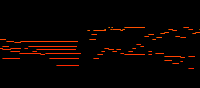
\includegraphics[width=\linewidth]{encode2.png}
					\caption{Encoding number 2.}
					\label{fig:encoded-2}
				\end{figure}
			\item The third encoding is a one-channeled version of the second one, where we doesn't store the velocity and instrument. This encoding was made only for testing the architecture with smaller dimensional inputs. This encoding is presented on figure \ref{fig:encoded-3}
				\begin{figure}[!htb]
					\centering
					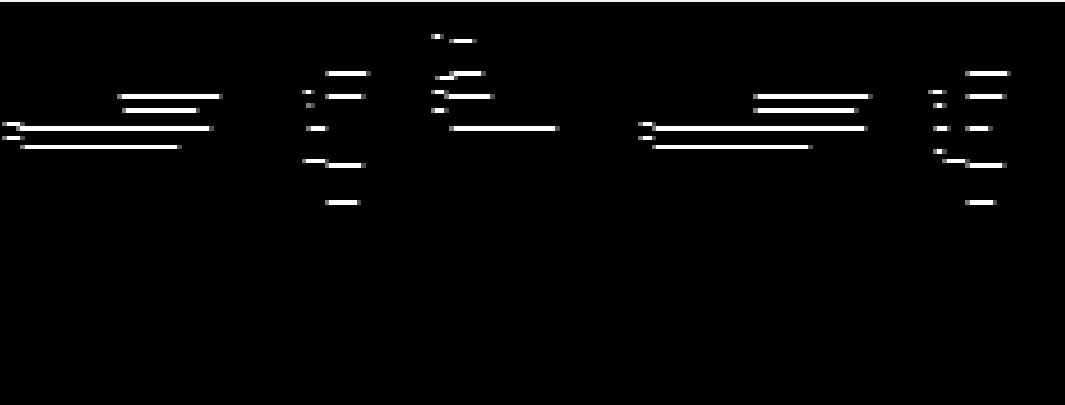
\includegraphics[width=\linewidth]{encode3.png}
					\caption{Encoding number 3.}
					\label{fig:encoded-3}
				\end{figure}
		\end{itemize}
	\end{enumerate}
	
	The code for the first encoding method can be found in \textbf{note2img.ipynb} notebook file, while the code for the second and third method can be found in \textbf{Midi2Img.ipynb} notebook file.
	\subsubsection{Decoding}
	
	After generating images with different Deep learning architectures it was necessary to create .midi files from the generated images. For this purpose we used two python packages: \textbf{Midifile} and \textbf{midiutil}. The pitch is represented on the y axis, and the duration of the note can be computed from the x axis in the following way: 
	
		\begin{gather}
		starting\_time = \frac{1000000 \times pixel\_sec \times staring\_pixel \times division}{tempo})) \\
		duration = \frac{1000000 \times length \times division}{tempo})), \\
		\text{where division is the same division which can be found in the MIDI header message} \nonumber
		\end{gather}
	
	Using the  \textbf{midifile.addNote(track, channel, note, time, duration, velocity)} function we could add notes easily to our midi files. \\ 
	
	The python code for the decoder can be found in \textbf{ImgToMidi.ipynb} notebook.
	
\subsection{Second approach - Hilbert's Curves}

Our first preprocessing approach produces pictures that are well-readable and understandable for humans. We were concerned however how well they can work with convolutional layers. The reason for our scepticism was that on real pictures the pixels tend to highly correlate with the other pixels in their surroundings. This can not be said about our preprocessing, which contains sudden changes. We implemented another method using Hilbert’s curves. In a nuttshell: Hilbert’s curves~\cite{hilbert} is a way to map the 1Darray-like amplitudes of a song (which are stored by many music file) to a 2D picture, in such way, that the notes close to each other in the array will also be close on the 2D picture. This approach might work better with convolutional networks since the small kernels, parsing the picture can actually extract features that correlates more.

\subsubsection{Encoding}
The encoding was done by a rather simple, custom written, recursive (because of the recursive nature of Hilbert's curves) function, that expects a $4^x$ number of samples. Divides them equally into four groups and calls itself with each group, then places the resulting  $4$ matrices to their corresponding position, while rotating and mirroring the bottom $2$.

%\ref{fig:hilbert}
\begin{figure}[H]
	\centering
	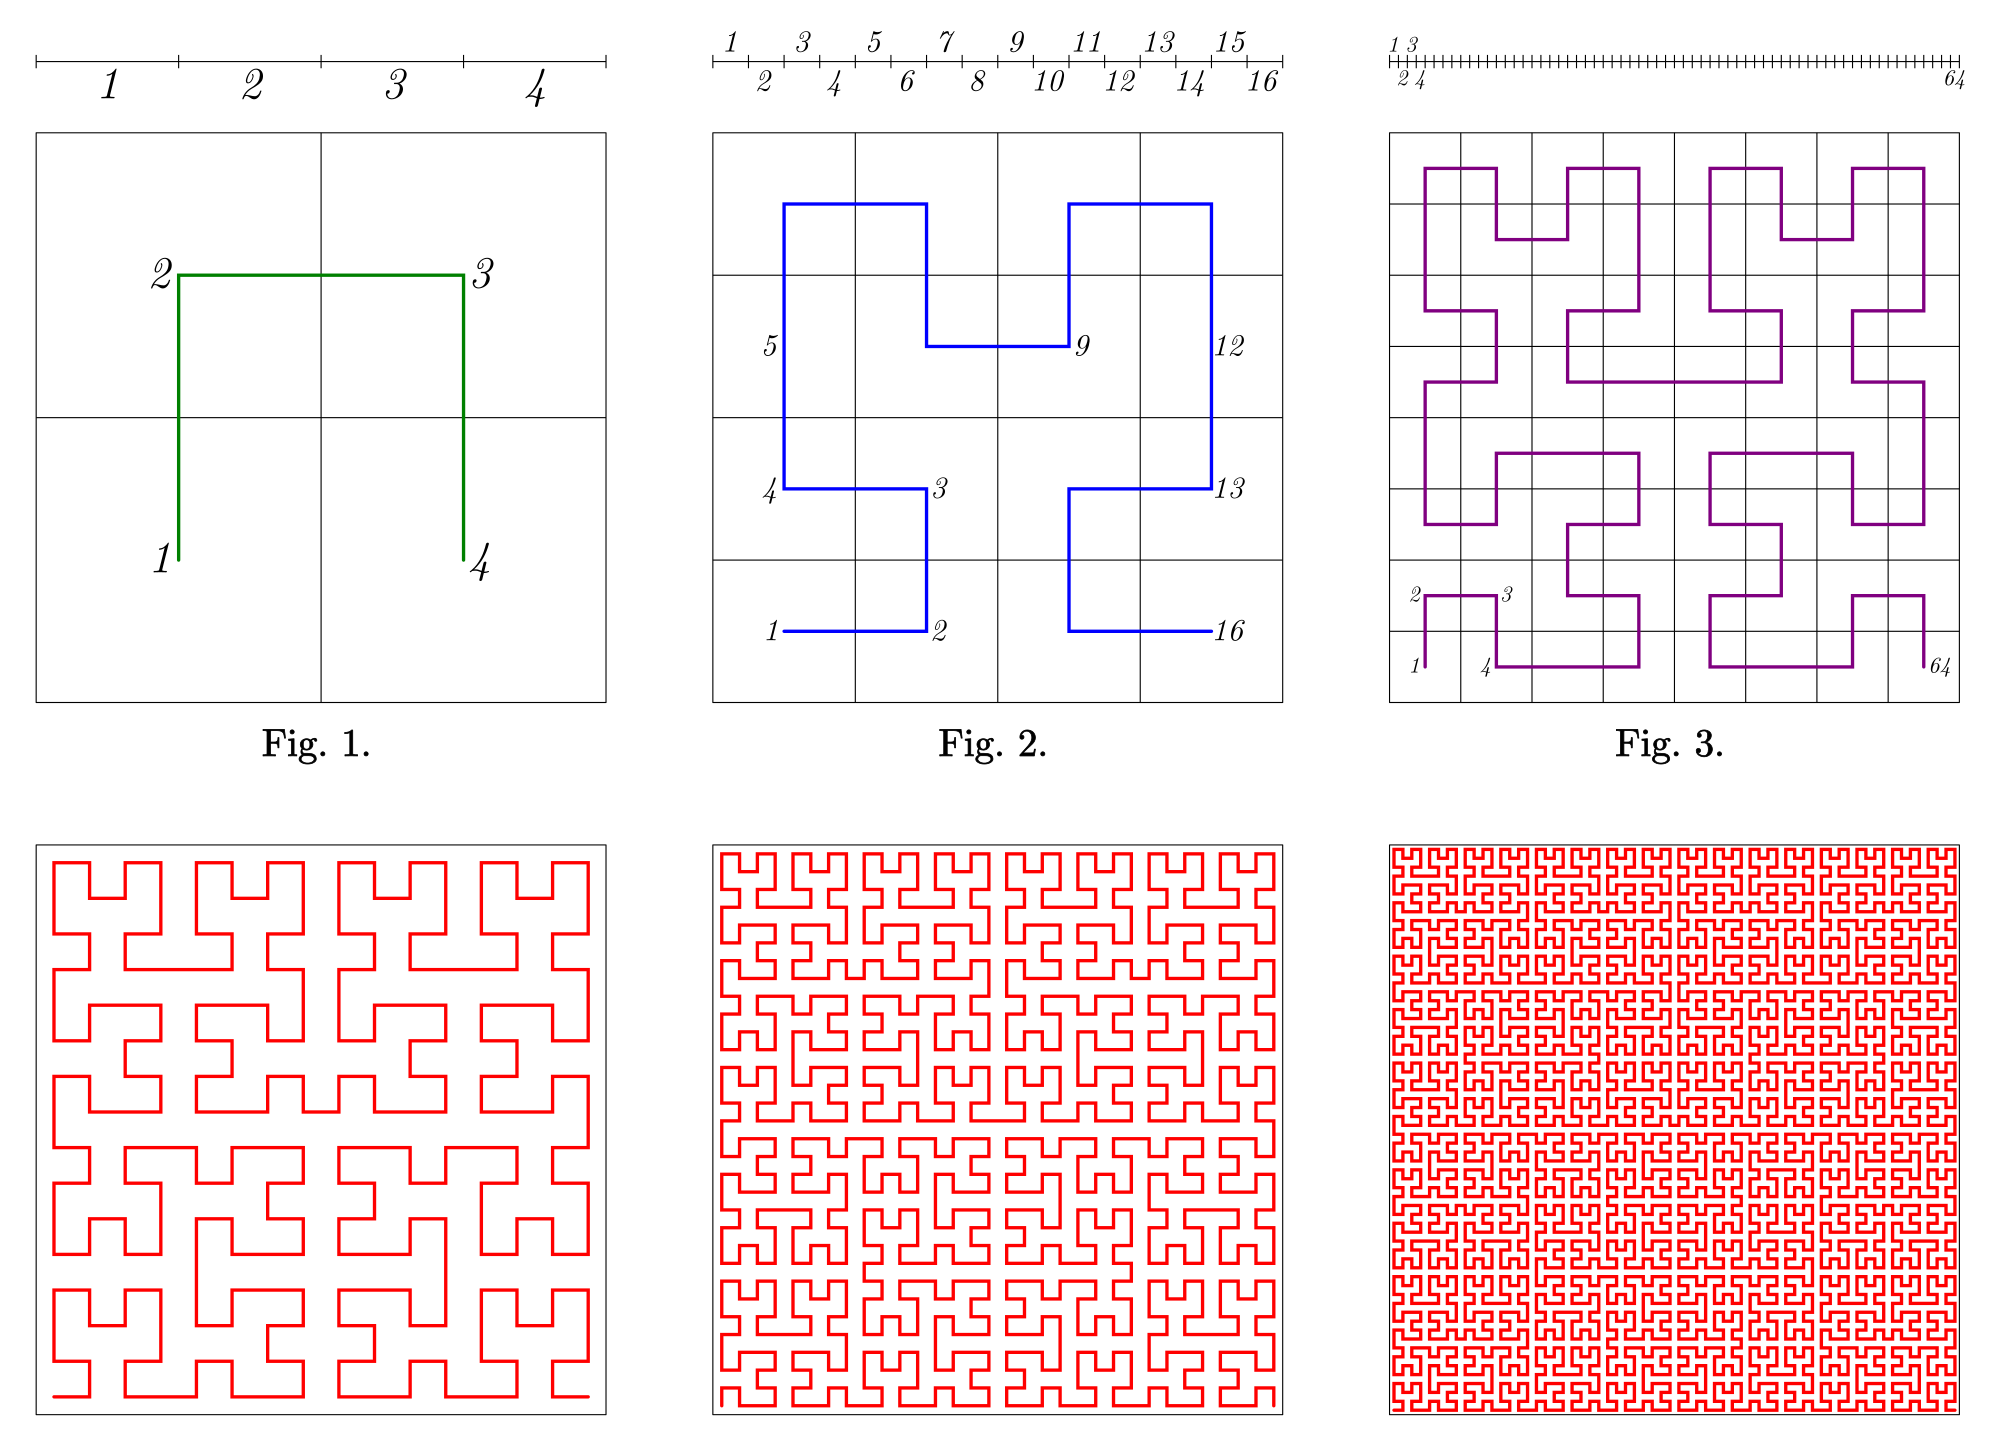
\includegraphics[width=\linewidth]{hilbert.png}
	\caption{Construction of more and more complex Hilbert curves.}
	\label{fig:hilbert}
\end{figure}

Obviously this approach does not work properly with the .midi files, thus we had to use their .wav version ($44100$Hz sampling rate, $2$ channels and $16$ bit values). We decided to use $256*256$ one channeled pictures (well technically they are not pictures but arrays). This means that on $1$ picture we can store $256*256/44100 = 1.49$ second long music. Might be worth adding, that we also scaled the resulting "pictures" to be between 0 and 1.

\subsubsection{Decoding}
The decoding is done by reversing the encoding. After it is done, we can write the 1D array into a .wav file and listen to the result.

\subsection{Data augmentaion - MIDI approach}

As we mentioned we used midi files collected in the MAESTRO dataset, but to widen our datas at our disposal we considered using two types of data augmentation methods: 
\begin{itemize}
	\item \textbf{Transposing music: } Before generating images from audio files we used an instrument called MIDICSV~\footnote{MIDICSV: Convert MIDI File to and from CSV - Fourmilab. \url{https://www.fourmilab.ch/webtools/midicsv/}}, which beside converting midi files to csv can also transpose music (shifting the whole melody to another key). So we could produce different (shifted along $Y$ axis) images from the same MIDI file.
	
	\item \textbf{Adding noise to music: } In the real life it is also possible that a musician makes mistakes while playing ( for example playes the wrong notes ). So therefore we also added a Gaussian noise to a few notes in the music. The expected value of the noise is 0 and the standard deviation is 1 (actually the noise is a standard normal distribution). We moved the note along the y axis by the integer value of the noise added to it.
\end{itemize}

\section{Network Architectures}
\label{sec:networksarch}

\subsection{Generative Adversarial Network (GAN)}
\label{sec;gan}

In our first attempt to generate music using images we tried to use some type of GAN network. This type of architechture uses 2 neural nets to work against each other in an adversarial manner. The first network is the generator takes noise as input and tries to generate a new image from it. The second network is the discriminator. The discriminators job is to learn the dataset and try to differentiate between the generated and the real images. Using the discriminators output as a metric for the generator to become better. The 2 networks should be trained after one another but not simultaneously. Since these networks take a long time to train and optimize we choose an off the shelf model. We used the GAN models found in Erik Linder-Norén's repository~\cite{} as reference. 
\subsubsection{Different GAN approaches.}
We tried to use the simple GAN model with the dataset mentioned in section~\ref{sec:data}. We didn't have much luck with this, the architechture seemed too simple to learn from our sparse dataset. Also this type of GAN is using Dense layers in the generator network, wich is not optimal to learn the structure of an image. The output was mostly noise with not much resemblance to the original dataset. 
\begin{figure}[!htb]
	\centering
	\caption{GAN generated output}
	\label{fig:gan}
\end{figure}
\section{DCGAN}
To compensate for the first models problems we settled on the DCGAN variant of the network. This type uses Deep Convolutional layers for both the generator and the discrimintator network. The idea was that convolution layers use a matrix of pixels as an input and it can learn the structure of an image much better. During the training this technique did work, however the generated outputs background was mostly gray and our images had black background. This made the discriminators job too easy and the loss didn't really converge to the expected values.
\begin{figure}[!htb]
	\centering
	
\includegraphics[width=\linewidth]{dcgan.png}
	\caption{DCGAN generated output.}
	\label{fig:dcgan}
\end{figure}
\section{WGAN GF}
The third approach was using WGAN GF found in paper~\cite{}. This uses a different method to calculate the error made by the generator network. This method seemed the most promising as the generated output started to look like the expected from around 2000 epochs. We let the network overfit our dataset so it would be as close to the original as possible. The output of the network can be seen in figure~\ref{fig:wgangf}.
\begin{figure}[!htb]
	\centering
	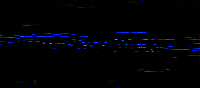
\includegraphics[width=\linewidth]{wgangf.png}
	\caption{WGAN GF generated output.}
	\label{fig:wgangf}
\end{figure}

\section{Style transformation using autoencoder}
As the project evolved we also wanted to achieve the style transformation of songs. For this purpose we created an autoencoder, that uses the Hilbert curve~\cite{hilbert} data preprocessing method. The idea was that if we teach our network with piano music only, it would learn how to restore piano music from the bottleneck. Our expectation was that after the learning is complete, if we use the autoencoder on non piano based music (in our case guitar) the network would transform the non piano input to piano music, since it only knows how to restore waves/amplitudes specific only to pianos. This was more or less achieved as you will possibly hear in our presentation, we believe that by fine-tuning the network (increase complexity while decreasing the bottleneck) it might be able to produce real, comfortable to listen to, piano transformed music.

\ref{fig:auto}
\begin{figure}[H]
	\centering
	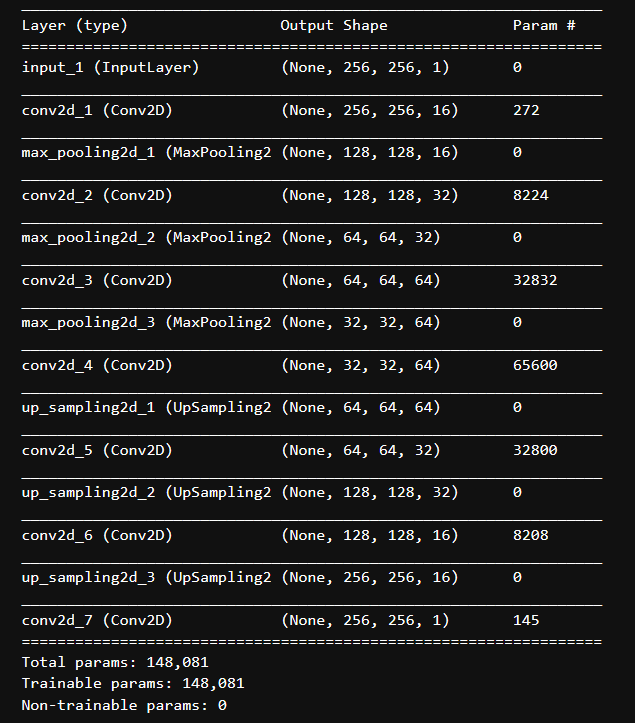
\includegraphics[width=0.7\linewidth]{auto_arch.png}
	\caption{Autoencoder architecture.}
	\label{fig:auto}
\end{figure}

\subsection{About the teaching of the AE}
At the beginning of the training we used ADAM optimizer with the following, default parameters (learningrate=0.001, beta1=0.9, beta2=0.999, amsgrad=False). With these the network learned relatively fast but unfortunately each try we experienced a sudden and huge increase in both validational and training loss, after which the network started to learn again (effectively negating all the training up until this point). To combat this effect we saved the best model ADAM produced, loaded it back and switched the optimizer to SGD with momentum. This did help the network to continue learning, however its speed considerably reduced (as expected).

\ref{fig:autores}
\begin{figure}[H]
	\centering
	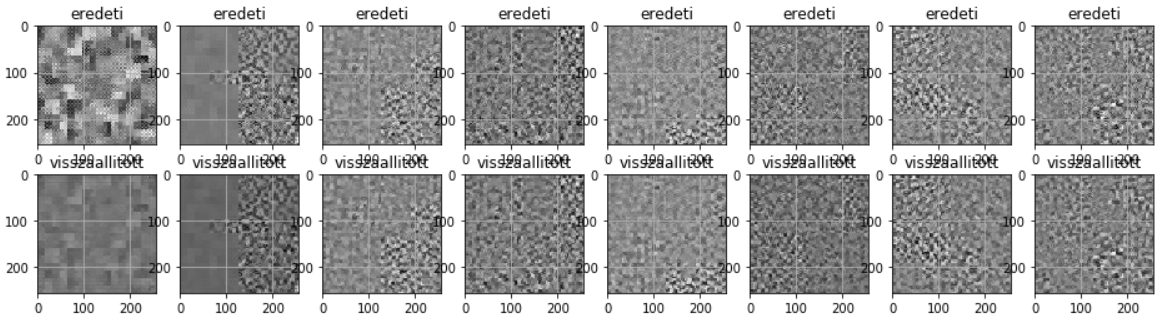
\includegraphics[width=\linewidth]{auto_results.png}
	\caption{Results of the AE with 1st row depicting the input, 2nd row depicting the output.}
	\label{fig:autores}
\end{figure}

\section{Long Short Term Memory (LSTM)}

As an alternative approach we tried to generate music using sequential recurrent architectures. We chose LSTM networks as the seed of this architecture. Long Short Term Memory networks are a special kind of RNN, capable of learning long-term dependencies. 
LSTMs are explicitly designed to avoid the long-term dependency problem. Remembering information for long periods of time is practically their default behavior, not something they struggle to learn. It was also a very promissing solution since in music generation it is very important to remember the long-term dependencies in the played music. The key to LSTMs is the cell state ($c$), runs straight down the entire chain, with only some minor linear interactions. It’s very easy for information to just flow along it unchanged (provides ability of remembering long-term dependencies). In addition an LSTM has three gates: input, output, forget gate, to protect and control the cell state. The structure of an LSTM cell can be seen on figure \ref{fig:lstmcell}

\begin{figure}[!htb]
	\centering
	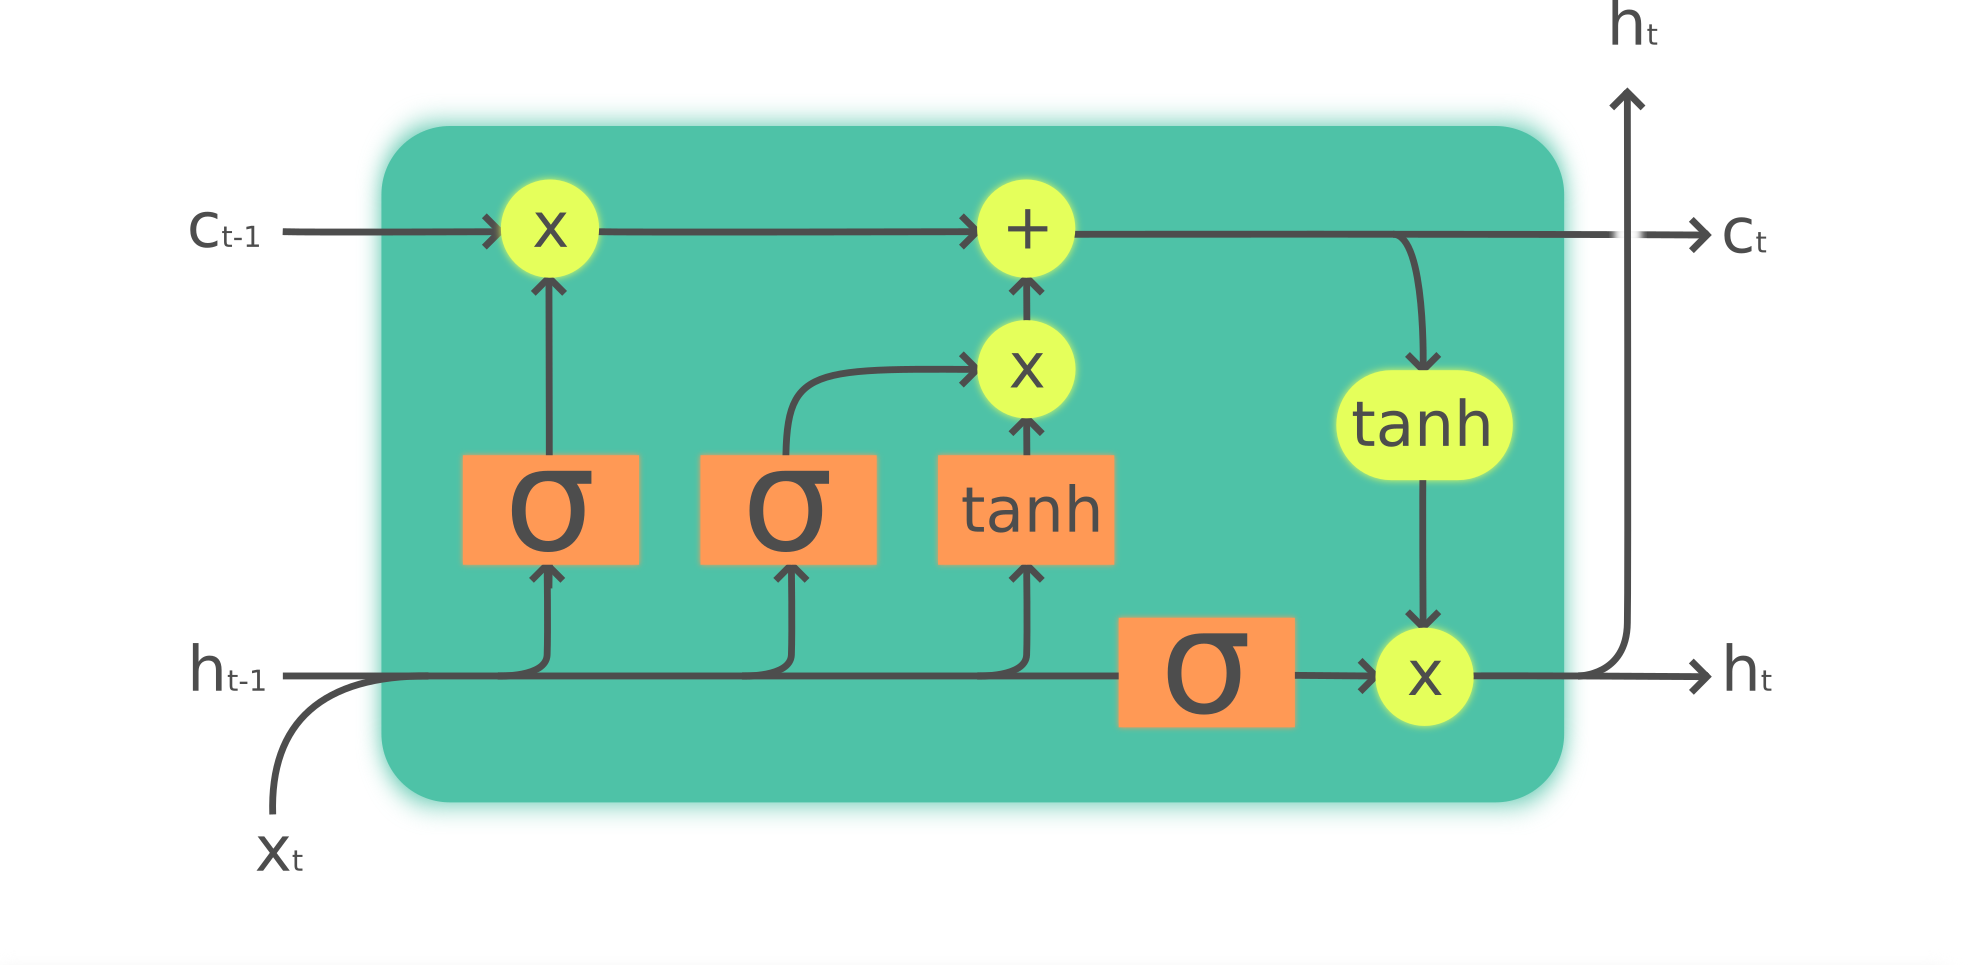
\includegraphics[width=\linewidth]{LSTMcell.png}
	\caption{Structure of an LSTM cell.}
	\label{fig:lstmcell}
\end{figure}

\subsection{Data generator}

Since had so many images that couldn't fit in memory we had to use a data generator to read images "batch-by-batch" into the memory. This generator is also practical becaouse it can easily produce fix length data sequences from the images, which is necessary if we want to train an LSTM. For the different LSTM architectures this generator was able to create data sequences with a shape of $[(batch, in\_seq, dim), (batch, out\_seq, dim)]$, where $in\_seq$ and $out\_seq$ are respectively the size of the input and output sequences, $dim$ is the dimension of a data point at one time stamp.  

\subsection{Training the basic LSTM model}

At first we tried to train a sequential model with only one LSTM layer with 128 neurons and with a Fully connected layer attached to its output. The structure of this model can be seen on figure \ref{fig:basicLSTMmodel}. 
\begin{figure}[!htb]
	\centering
	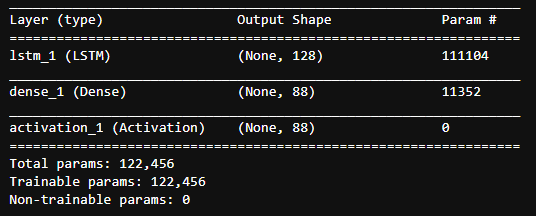
\includegraphics[width=0.8\linewidth]{basicLSTMmodel.png}
	\caption{Basic model with one LSTM layer.}
	\label{fig:basicLSTMmodel}
\end{figure}

The output is a vector corresponding to one column in the generated image (that's why the size of this vector is 88, which is the heigth of the image). 

\subsubsection{Teacher forcing}
Teacher forcing is a technique applied in the training process of a recurrent neural network where the target data (the ground truth) is passed as the next input to the RNN independent on what was the network's previous prediction. 
Using this method during the training we passed to LSTM 100 columns of an image as input data sequence and we expected to get the next column of the image as the predicted output. 
As testing procedure we gave a seed as the input of the LSTM (a 100 wide data sequence from the real images) and the LSTM generated the next few columns/time stamps of the music.
We tried to train this model on the dataset created by the first encoding presented in the section \ref{sec:prepoc}. This encoding was too sparse for this LSTM, it learned quickly to generate totally black images without painting any colour pixels onto it. 

After training it on the dataset created by the second encoding process (using Teacher forcing) the results started to become a bit different from the first training. However it generated noisy images (as the one presented on figure \ref{fig:LSTMresult-1}). The first half of the image is the seed and the second (noisy) part is the generated part. 

\begin{figure}[!htb]
	\centering
	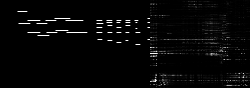
\includegraphics[width=\linewidth]{LSTMresult1.png}
	\caption{Result using Teacher forcing on basic LSTM.}
	\label{fig:LSTMresult-1}
\end{figure}

\subsubsection{Custom loss function}

At the basic LSTM model we used Mean-Squared Error as loss function, but since that model generated very noise images we considered creating a custom loss function which is able to reduce the noise on the output. 

Each value stored in pixel channels are real numbers from the [0, 1] intervall. That is $y\_true$ the expected output is also in this range. In this case: 

\begin{gather}
\lim_{x\to\infty} \sqrt[x]{y\_true} = 1, \text{for every $y\_true > 0$ value}
\end{gather}

Now let's consider the following loss function: 
\begin{gather}
	C(y) = \lim_{x\to\infty} \frac{1}{M}\sum_{i = 0}^{M} \alpha(y_i - \sqrt[x]{y\_true_i})^{2}\sqrt[x]{y\_true_i} + \beta(y_i - \sqrt[x]{y\_true_i})^{2}(1 - \sqrt[x]{y\_true_i}), \\
	\text{where $M$ is the number of datapoints}
\end{gather}

It can be seen that by adjusting the $\alpha$ and $\beta$ parameters we can influence how the model punishes the following two cases: 
\begin{itemize}
	\item $y\_true$ is close to 1 and $y$ is close to zero (this can be influenced by setting $\alpha$)
	\item $y\_true$ is 0 and $y$ is close to one (this can be influenced by setting $\beta$)
\end{itemize}

With $\alpha = 1.5$ and $\beta = 0.8$ we got the result presented on figure \ref{fig:LSTMresult-2}

\begin{figure}[!htb]
	\centering
	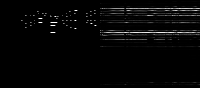
\includegraphics[width=\linewidth]{LSTMresult2.png}
	\caption{Result using Teacher forcing on LSTM with custom loss.}
	\label{fig:LSTMresult-2}
\end{figure}

We noticed that after applying our custom loss function the noise along y axis disappeared, the network learned to continue the music in the same note interval as it was in the seed, it doesn't generate too high or two low notes. But also it can be seen that the network still doesn't know when to stop playing a specific note (the pixel intensity fades away along x axis instead separating notes by black pixels) 

As a possible solution to this problem we tried to use the encoder-decoder based Seq2seq LSTM architecture and we stopped using Teacher forcing during the training process. 

\subsection{Seq2seq LSTM}

Seq2seq models are used to generate output with various length from variable length input data sequence. In these models usually there is an encoder RNN which creates an interpretation of the input sequence and passes it to the decoder network, which also has its own input besides the information got from encoder. The output of the decoder will be the generated data. The structure of a Seq2seq model can be seen on figure \ref{fig:seq2seqmodel}

\begin{figure}[!htb]
	\centering
	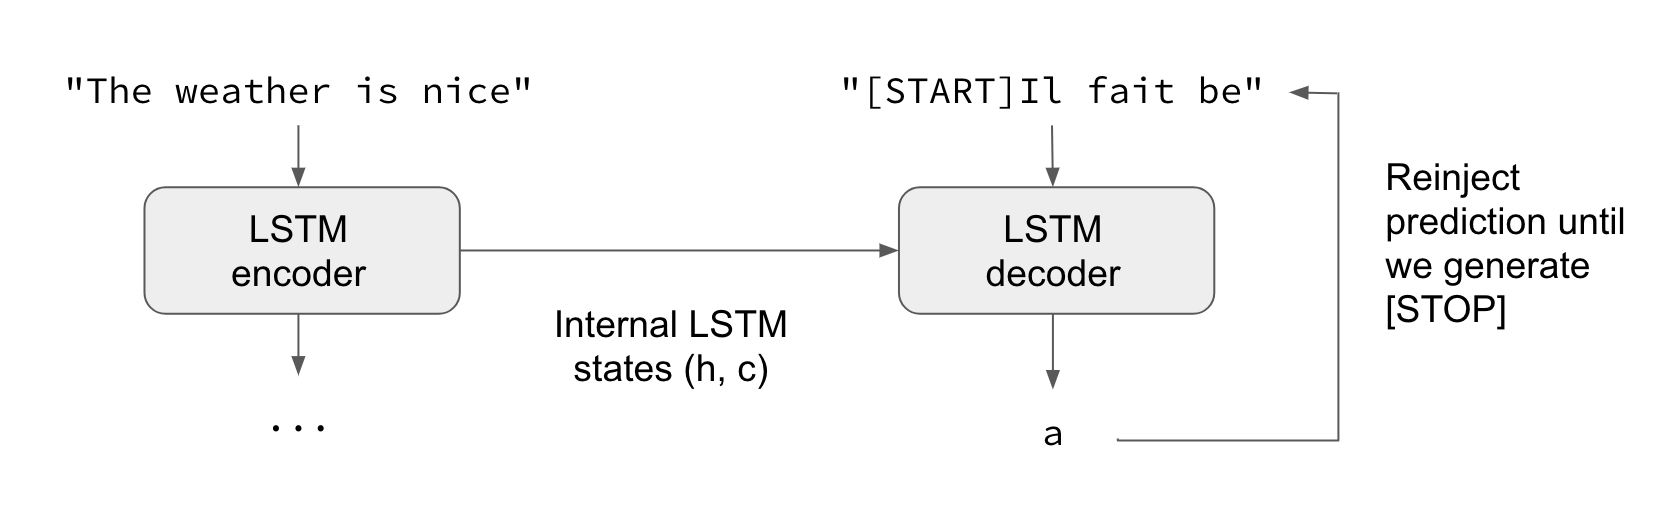
\includegraphics[width=\linewidth]{seq2seqmodel.png}
	\caption{Seq2seq model structure}
	\label{fig:seq2seqmodel}
\end{figure}

We applied LSTM cells as the seed of this seq2seq model. Instead of using keras's built-in Sequential model, we used Functional model so we could realize the generation of variable output sequence. The structure of our custom built seq2seg model can be seen on figure \ref{fig:seq2seqsummary}
\begin{figure}[!htb]
	\centering
	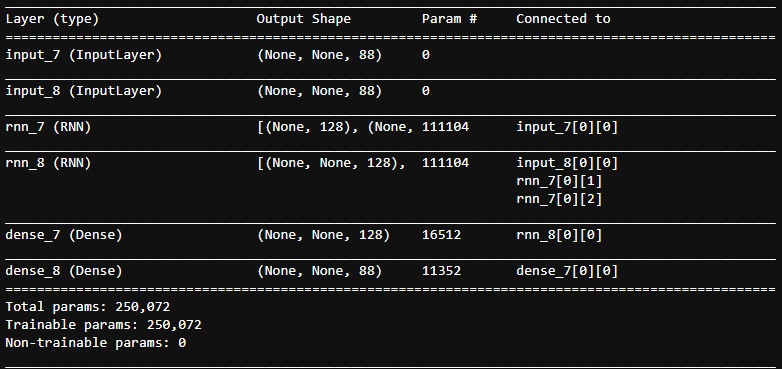
\includegraphics[width=\linewidth]{seq2seqsummary.png}
	\caption{Seq2seq model summary}
	\label{fig:seq2seqsummary}
\end{figure}
In both the encoder and decoder network we put an LSTMCell into an RNN layer. In case of the encoder the number of unfolded time steps during training are equal to the length of input data sequence. Similarly in case of the decoder the number of unfolded time steps are equal to the length of output sequence.
On of the advantages of this model is that it can learn to predict multiple future output in contrast of Teacher forcing method which was trained to predict only one column of the input image using the previous columns. 
We trained this model to generate the next 10 and 100 columns (time steps) of the music based on the previous 100 columns (which corresponds to approximatelly 5 seconds of music). The results can be seen on figure \ref{fig:seq2seqresult1}.

\begin{figure}[!htb]
	\centering
	\caption{Predicting 100 columns}{
		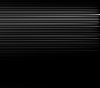
\includegraphics[width=0.48\linewidth]{seq2seqresult1.png}}
	\label{fig:seq2seqresult1}
\end{figure}

The played notes are separated by black lines, which is a good sign: the model learned to distinguish different pitches. But the "white" lines are fading away here also, which means that the model couldn't learn the possible discrete values of the encoding. 

To resolve this problem we considered transforming this into a kind of classification problem: the network needs to predict the class of each pixel of the next column of the image: is it a "silent" (black), "note started" (125/255 intensity gray) or "note sustained" (white) pixel. This classification problem can be realized with a categorical cross entropy loss function and softmax activations at the output fully connected layers. 

Another possible direction for further researches can be using bi-directional LSTM cells instead of basic LSTM-s. 

\subsubsection*{Acknowledgments}

Use unnumbered third level headings for the acknowledgments. All
acknowledgments go at the end of the paper. Do not include
acknowledgments in the anonymized submission, only in the final paper.

\section*{References}

References follow the acknowledgments. Use unnumbered first-level
heading for the references. Any choice of citation style is acceptable
as long as you are consistent. It is permissible to reduce the font
size to \verb+small+ (9 point) when listing the references. {\bf
  Remember that you can use a ninth page as long as it contains
  \emph{only} cited references.}
\medskip

\small

\newpage

\tableofcontents
%\spacing{1.5}
\newpage

\end{document}